% CVPR 2022 Paper Template
% based on the CVPR template provided by Ming-Ming Cheng (https://github.com/MCG-NKU/CVPR_Template)
% modified and extended by Stefan Roth (stefan.roth@NOSPAMtu-darmstadt.de)

\documentclass[10pt,twocolumn,letterpaper]{article}

%%%%%%%%% PAPER TYPE  - PLEASE UPDATE FOR FINAL VERSION
% \usepackage[review]{cvpr}      % To produce the REVIEW version
\usepackage{cvpr}              % To produce the CAMERA-READY version
%\usepackage[pagenumbers]{cvpr} % To force page numbers, e.g. for an arXiv version

% Include other packages here, before hyperref.
\usepackage{graphicx}
\usepackage{amsmath}
\usepackage{amssymb}
\usepackage{booktabs}
\usepackage{multirow}
\usepackage{todonotes}

% It is strongly recommended to use hyperref, especially for the review version.
% hyperref with option pagebackref eases the reviewers' job.
% Please disable hyperref *only* if you encounter grave issues, e.g. with the
% file validation for the camera-ready version.
%
% If you comment hyperref and then uncomment it, you should delete
% ReviewTempalte.aux before re-running LaTeX.
% (Or just hit 'q' on the first LaTeX run, let it finish, and you
%  should be clear).
\usepackage[pagebackref,breaklinks,colorlinks]{hyperref}


% Support for easy cross-referencing
\usepackage[capitalize]{cleveref}
\crefname{section}{Sec.}{Secs.}
\Crefname{section}{Section}{Sections}
\Crefname{table}{Table}{Tables}
\crefname{table}{Tab.}{Tabs.}


%%%%%%%%% PAPER ID  - PLEASE UPDATE
\def\cvprPaperID{*****} % *** Enter the CVPR Paper ID here
\def\confName{CVPR}
\def\confYear{2022}


\begin{document}

%%%%%%%%% TITLE - PLEASE UPDATE
\title{A Comparison of Actor Critic and Policy Gradient \\ Algorithms for Learning Mechanical Designs}

\author{Andrew Albright \& Adam Smith\\
University of Louisiana at Lafayette\\
104 E. University Circle, Lafayette, LA 70503\\
{\tt\small andrew.albright1@louisiana.edu, adam.smith2@louisiana.edu}
% For a paper whose authors are all at the same institution,
% omit the following lines up until the closing ``}''.
% Additional authors and addresses can be added with ``\and'',
% just like the second author.
% To save space, use either the email address or home page, not both
% \and
% Second Author\\
% University of Louisiana at Lafayette\\
% 104 E. University Circle, Lafayette, LA 70503\\
% {\tt\small secondauthor@i2.org}
}
\maketitle

\listoftodos

%%%%%%%%% ABSTRACT
\begin{abstract}
  Legged systems have many advantages when compared to their wheeled counterparts. For example, they can more easily navigate extreme, uneven terrain. However, there are disadvantages as well, particularly the difficulty seen in modeling the nonlinearities of the system. Research has shown that using flexible components within legged locomotive systems improves performance measures such as efficiency and running velocity. Tuning mechanical designs to define what might be an optimal performing system is challenging though, particularly when the system is nonlinear. Reinforcement learning can be tasked with learning mechanical parameters of a system to match a control input. It is shown in this work that when deploying reinforcement learning to find design parameters for a monopode jumping system, the designs the algorithms learn are optimal within the design space provided to the agents.
\end{abstract}

%%%%%%%%% BODY TEXT
%------------------------------------------------------------------------
\section{Introduction}
\label{sec:intro}

The use of flexible components within legged locomotive systems has proved useful for both reducing power consumption and increasing performance \cite{Sugiyama2004, Buondonno2017, Hurst2008}. However, designing controllers for these systems is difficult as the flexibility of the system generates nonlinear models. As such, employing series-elastic-actuators (SEA) instead of flexible links is an attractive and popular solution, since the models of the systems become more manageable \cite{Buondonno2017, Zhang2019, Pratt1995}. Still, the use of SEAs do not represent the full capability of flexible systems. As a result, other methods that use flexible tendon-like materials meant to emulate more organic designs have been proposed \cite{Iida2005}. These, however, are still not representative of fully flexible links, which have been shown to drastically improve locomotive performance measures such as running speed \cite{Saranli2001}.

Control methods have been developed that work well for flexible systems like the ones mentioned \cite{Luo1993, Modeling2003}. However, as the systems increase in dimensionality, effects such as dynamic coupling between members make such methods challenging to implement. As such, work has been done that uses neural networks and methods such as reinforcement learning (RL) to develop controllers for flexible systems \cite{Bhagat2019e, Thuruthelb}. For example, RL has been used to create control strategies for both flexible-legged and rigid locomotive systems that when compared, show the locomotive systems outperform their rigid counterparts \cite{Dwiel2019d}. Furthermore, those controllers were shown to be robust to changes in design parameters. 

In addition to the work done using RL to develop controllers for flexible systems, work has been completed which shows that this technique can be used to concurrently design the mechanical aspects of a system and a controller to match said system \cite{Ha2019j}. These techniques have even been used to define mechanical parameters and control strategies where the resulting controller and hardware were deployed in a sim-to-real process, validating the usability of the technique \cite{Chen2020}. Using this technique for legged-locomotion has also been studied, but thus far has been limited to the case of rigid systems \cite{Schaff2019e}. 

As such, this paper explores the use of RL for concurrent design of flexible-legged locomotive systems. A simplified flexible jumping system was used where, for the initial work, the control input was held fixed so that an RL algorithm was tasked with only learning optimized mechanical parameters. The rest of the paper is organized such that in the next section, similar work will be discussed. In Section \ref{sec:monopode_model}, the monopode environment details will be defined. Next, in Section~\ref{sec:control_input_exp}, the input used during training will be explained. Then, in Section~\ref{sec:learning_mech_params}, the algorithm used along with the method of the experiments will be presented. The performance of the learned designs are shown in Section~\ref{sec:results}.

%%%%%%%%% RELATED WORK

\section{Related Work}
\label{sec:related_work}
\subsection{Flexible Locomotive Systems}

The use of flexible components within locomotive robotics systems has shown improvements in performance measures such as movement speed and jumping height \cite{Sugiyama2004, Hurst2008}. Previous work has shown that the use of flexible components in the legs of legged locomotion systems increase performance while decreasing power consumption \cite{Saranli2001}. Research also has been done showing the uses of series-elastic-actuators for locomotive systems \cite{Pratt1995}. In much of this work, human interaction with the robotic systems is considered such that rigidity is not ideal \cite{Zhang2019}. The studies of flexible systems are challenging however, as the models which represent them are often nonlinear and therefore difficult to develop control systems for. As such, finding optimal mechanical designs is challenging and often times overlooked. 

\subsection{Controlling Flexile Systems Using RL}

Control methods developed for flexible systems have been shown to be effective for position control and vibration reduction \cite{Luo1993, Ahmadi1997}. Because of the challenges seen in scaling the controllers, methods utilizing reinforcement learning are of interest. This method has been used in simple planar cases, where it was compared to a PD control strategy for vibration suppression and proved to be a higher performing method \cite{He2020f}. Additionally, it has also been shown to be effective at defining control strategies for flexible-legged locomotion. The use of actor-critic algorithms such as Deep Deterministic Policy Gradient \cite{Lillicrap2016h} have been used to train running strategies for a flexible legged quadruped \cite{Dwiel2019d}. Much of the research is based in simulation, however, and often the controllers are not deployed on physical systems, which leads to the question of whether or not these are useful techniques in practice.

\subsection{Concurrent Design}

Defining an optimal controller for a system can be difficult due to challenges such as mechanical and electrical design limits. This is especially true when the system is flexible and the model is nonlinear. A solution to this challenge is to concurrently design a system with the controllers so that the two are jointly optimized. This strategy has been used to develop better performing mechatronics systems \cite{Li2001}.  More recent work has used advanced methods such as evolutionary strategies to define robot design parameters \cite{Wang2019}. In addition to evolutionary strategies, reinforcement learning has been shown to be a viable solution for concurrent design of 2D simulated locomotive systems \cite{Ha2019j}. This is further shown to be a viable method by demonstrating more complex morphology modifications in 3D reaching and locomotive tasks \cite{Schaff2019e}. However, these techniques have not yet been applied to flexible systems for locomotive tasks. 

%%%%%%%%% MONOPODE MODEL

\section{Monopode Model}
\label{sec:monopode_model}

The monopode model in Figure~\ref{fig:monopode} has been shown to be useful for creating a simplified representation of many animal based running and jumping gaits \cite{Blickhan1993a}. As such, it is used in this work to demonstrate the ability of reinforcement learning for the mechanical design aspect of concurrent design. The model parameters used in the simulations in this paper are summarized in Table~\ref{tab:monopode}.
%
The variable $m_a$ represents the mass of the actuator, which moves along the rod of mass $m_l$. A nonlinear spring shown in the figure by constant $\alpha$ is used to represent flexibility within the jumping system. A damper (not shown in Figure~\ref{fig:monopode}), is parallel to the spring. Variables $x$ and $x_a$ represent the vertical position of the system with respect to the ground and the position of the actuator along the rod, respectively.
	
The equations of motion describing the system are:
%	
\begin{equation}
		\ddot{x} = \frac{\gamma}{m_t} \left(\alpha\,x + \beta\,x^3 + c\,\dot{x}\right)-\frac{m_a}{m_t}\,\ddot{x}_a-g
\end{equation}
%
where $x$ and $\dot{x}$ are position and velocity of the rod, respectively, the acceleration of the actuator, $\ddot{x}_a$, is the control input, and $m_t$ is the mass of the complete system. Constants $\alpha$ and $c$ represent the nonlinear spring and damping coefficient, respectively, and constant $\beta$ is set to $1e8$. Ground contact determines the value of $\gamma$, so that the spring and damper do not supply force while the leg is airborne:
%
	\begin{equation}
		\gamma =
		\left\{\begin{matrix}
		   -1, & x \leq 0\\ 
		   \hphantom{-} 0, & \mbox{otherwise}
		   \end{matrix}\right.
                %    \vspace{.25cm}
	 \end{equation}
%

Additionally, the system is constrained such that it only moves vertically and the spring can only compress a certain amount. In this work the spring is allowed to compress the same distance that the actuator can move, which is 0.008~m.

%
\begin{figure}[t]
        \begin{center}
        \includegraphics[width=2.5cm]{figures/Monopode_System/monoped.png}
        \caption{Monopode System}
        \label{fig:monopode} 
        \end{center}
        % \vspace{-4mm}
        \end{figure}
        %
\begin{table}[t]
        \caption{Monopode Model Parameters}
        \vspace{-4mm}
        \label{tab:monopode}
        \begin{center}
                \begin{tabular}{|c||c|}
                %			& & \\ % put some space after the caption
                \hline
                \textbf{Model Parameter} & \textbf{Value}\\
                \hline
                Mass of Leg, $m_l$                                       & 0.175 kg                                          \\
                Mass of Actuator, $m_a$                                  & 1.003 kg                                          \\
                Spring Constant, $\alpha_{nominal}$                      & 5760 $\textup{N}/\textup{m}$                      \\
                Natural Frequency, $\omega_n$                            & $\sqrt{\frac{\alpha}{m_l + m_a}}$                 \\
                Damping Ratio, $\zeta_{nominal}$                         & 1e-2 \& 7.5e-2 $\frac{\textup{N}}{\textup{m/s}}$  \\
                % Damping Constant, $c$                                    & $2 \, \zeta \, \omega_n m$                        \\
                \hline
                Actuator Stroke, $(x_{a})_{\textup{max}}$                & 0.008 $\textup{m}$                                \\
                Max.\ Actuator Velocity, $(\dot{x}_{a})_{\textup{max}}$  & 1.0 $\textup{m}/\textup{s}$                       \\ 
                Max.\ Actuator Accel., $(\ddot{x}_{a})_{\textup{max}}$   & 10.0 $\textup{m}/\textup{s}^2$                    \\
                \hline
                \end{tabular}
        \end{center}
        % \vspace{-5mm}
\end{table}
% 
        
%%%%%%%%% COMMAND DESIGN

\section{Jumping Command Design}
\label{sec:control_input_exp}

Bang-bang based jumping commands like the one shown in Figure \ref{fig:sim_command} are likely to result in a maximized jump height \cite{Vaughan2013}. For this command, the actuator mass travels at maximum acceleration within its allowable range, pauses, then accelerates in the opposite direction. Commands designed to complete this motion are bang-bang in each direction, with a selectable delay between them. The resulting motion of the actuator along the rod is shown in Figure \ref{fig:command_act_motion}. Starting from an initial position, $(x_a)_0$, it moves through a motion of stroke length $\Delta_1$, pauses there for $\delta_t$, then moves a distance $\Delta_2$ during the second portion of the acceleration input.

%
\begin{figure}[tb]
\begin{center}
\includegraphics[width = 3in]{figures/input_shaping/Command_form.pdf}  
\caption{Jumping Command}
\label{fig:sim_command}
\end{center}
% \vspace{-4mm}
\end{figure}
%
%
\begin{figure}[tb]
\begin{center}
\includegraphics[width = 3in]{figures/input_shaping/Jumping_command_position.pdf}  
\caption{Resulting Actuator Motion}
\label{fig:command_act_motion}
\end{center}
% \vspace{-4mm}
\end{figure}
%

This bang-bang-based profile can be represented as a step command convolved with a series of impulses, as shown in Figure \ref{fig:jump_convolve} \cite{Sorensen2008CommandinducedVA}. Using this decomposition, input-shaping principles and tools can be used to design the impulse sequence \cite{Singer:90, Singhose:94a}. 
%
\begin{figure}[tbp]
\begin{center}
\includegraphics[width = 3.0in]{figures/input_shaping/Jump_convolve.pdf}
\caption{Decomposition of the Jump Command into a Step Convolved with an Impulse Sequence}
\label{fig:jump_convolve}
\end{center}
% \vspace{-4mm}
\end{figure}
%
For the bang-bang-based jumping command, the amplitudes of the resulting impulse sequence are fixed, $A_i = [-1, 2, -1, 1, -2, 1]$. The impulse times, $t_i$, can be varied and optimal selection of them can lead to a maximized jump height of the monopode system \cite{Vaughan2013}. Commands of this form will often result in a stutter jump like what is shown in Figure~\ref{fig:stutter_jump}, where the small initial jump allows the system to compress the spring to store energy to be used in the final jump. This jumping command type was used as the input for the monopode during the simulation phase of training.
%
\begin{figure}[t]
        \begin{center}
        \includegraphics[width=3in]{figures/Monopode_System/stutter_jump.png}
        \caption{Example Stutter Jump}
        \label{fig:stutter_jump} 
        \end{center}
        % \vspace{-4mm}
\end{figure}

%%%%%%%%% MECHANICAL DESIGN

\section{Learning Mechanical Design}
\label{sec:learning_mech_params}
\subsection{Reinforcement Learning Algorithm}
%
Two different algorithms are used and compared in this work for finding mechanical design parameters. They are the Twin Delayed Deep Deterministic Policy Gradient (TD3) and the Proximal Policy Optimization (PPO) algorithm \cite{Fujimoto2018d, Schulman2017f}. A comparison of actor-critic and policy gradient based algorithms will be shown such that one might be selected in future work for implementing a fully concurrent design process. The StableBaselines3 implementation of the algorithms was used as they are well written, popular in research, and thoroughly documented \cite{stable-baselines3}.

The training hyperparameters were selected based on the algorithm author recommendations and StableBaselines3 experimental findings. The vales are displayed in Table~\ref{tab:training_hyperameters}. All of the hyperparameters, with the exception of the rollout (Learning Starts) and the replay buffer, were set according to StableBaselines3 standards. The rollout setting was defined such that the agent could search the design space at random, filling the replay buffer with enough experience to prevent the agent from converging to a design space that was not optimal. The replay buffer was sized proportional to the number of training steps due to system memory constraints.  
%
\begin{table}[t]
        \caption{TD3 Training Hyperparameters}
        \vspace{-4mm}
        \label{tab:training_hyperameters}
        \begin{center}
        \begin{tabular}{|c||c|}
        \hline
        Hyperparameter                     & Value                           \\
        \hline
        Learning Rate, $\alpha$         & 0.001                           \\
        Learning Starts                 & 100 Steps                       \\
        Batch Size                      & 100 Transitions                 \\
        Tau, $\tau$                     & 0.005                           \\
        Gamma, $\gamma$                 & 0.99                            \\
        Training Frequency              & 1:Episode                       \\
        Gradient Steps                  & $\propto$ Training Frequency    \\
        Action Noise,  $\epsilon$       & None                            \\
        Policy Delay                    & 1 : 2 Q-Function Updates        \\
        Target Policy Noise, $\epsilon$ & 0.2                             \\
        Target Policy Clip, $c$         & 0.5                             \\
        Seed                            & 100 Random Seeds                \\
        \hline
        \end{tabular}
        \end{center}
        \vspace{-5mm}
\end{table}
%
%
\begin{table}[t]
        \caption{PPO Training Hyperparameters}
        \vspace{-4mm}
        \label{tab:training_hyperameters_PPO}
        \begin{center}
        \begin{tabular}{|c||c|}
        \hline
        Hyperparameter                  & Value                           \\
        \hline
        Learning Rate, $\alpha$         & 0.001                           \\
        Batch Size                      & 64                              \\
        Clip Range, $\epsilon $         & 0.2                             \\
        Gamma, $\gamma$                 & 0.99                            \\
        GAE-Lambda,                     & 0.95                            \\
        Training Frequency              & 1:Episode                       \\
        Gradient Steps                  & $\propto$ Training Frequency    \\
        Policy Delay                    & 1 : 2 Q-Function Updates        \\
        Target Policy Noise, $\epsilon$ & 0.2                             \\
        Target Policy Clip, $c$         & 0.5                             \\
        Seed                            & 100 Random Seeds                \\
        \hline
        \end{tabular}
        \end{center}
        \vspace{-5mm}
\end{table}
%

The training hyperparameters for PPO found in Table~\ref{tab:training_hyperameters_PPO} were set similarly to TD3's. All the PPO hyperameters, other than learning rate and N-steps, were set according to the algorithm's author and StableBaselines3's recommendations.
The learning rate and N-steps were adjusted as the algorithm was not able to converge within 1000 episodes given the initial hyperparameter values of 0.0003 and 2048. The learning rate and N-steps parameters were selected such that results converged in a similar amount of
episodes as TD3.

\subsection{Training Environment Design}
%
To allow the agent to find a mechanical design, a reinforcement learning environment conforming to the OpenAI Gym standard \cite{Brockman2016c} was created for the monopode model described in Section~\ref{sec:monopode_model}, including a fixed controller input based on the algorithm described in the previous section. Unlike the common use case for RL, which is tasking the agent with finding a control input to match a design, the agent in this work was tasked with finding mechanical parameters to match a control input.

The mechanical parameters the agent was tasked with optimizing were the spring constant and the damping ratio of the monopode system. At each episode during training, the agent selected a set of design parameters from a distribution of available designs and a simulation was run with those parameters and a fixed control input. The actions applied, $\mathcal{A}$, and transitions saved, $\mathcal{S}$, from the environment were defined as follows:
%
\begin{equation}
        \label{eq:action}
        \begin{aligned}
        \mathcal{A} = \{ \{ a_{\alpha} \in \mathbb{R}: [0.1 \alpha, 1.9 \alpha] \}, \\ 
        \{ a_{\zeta} \in \mathbb{R}: [0.1 \zeta, 1.9 \zeta] \} \}
        \end{aligned}
\end{equation} 
%
\begin{equation}
        \label{eq:transitions}
        \mathcal{S}= \left \{ \textbf{X}, \, \dot{\textbf{X}}, \, \textbf{X}_a, \, \dot{\textbf{X}_a}  \right \}
\end{equation}
%
where $\alpha$ and $\zeta$ are the nominal spring constant and damping ratio of the monopode, respectively; $x_t$ and $\dot{x}_t$ are the rod height and velocity steps of the monopode, and $x_{at}$ and $\dot{x}_{at}$ are the actuator position and velocity steps of the monopode, all captured during simulation. 

\subsection{Reward Function Design}

The RL algorithm was utilized to find designs for two different reward cases. Time series data was captured during the simulation phase of training and was used to evaluate the designs performance through these rewards. The first reward case used was:
%
\begin{equation}
        \mathbb{R}_1 = \left (\textbf{X}  \right )_{\text{max}}
\end{equation}
% 
where $\textbf{X}$ was the timeseries rod height of the monopode captured during simulation. The goal of the first reward was to find a design that would cause the monopode to jump as high as possible.

The reward for the second case was:
%
\begin{equation}
        \mathbb{R}_2 = - \frac{\left (\textbf{X}  \right )_{\text{max}} - x_{s}}{x_{s}}
\end{equation}
%
where $x_s$ was the desired jump height, which was set to 0.1~m. The second case was utilized to test RL's ability to find a design that minimized the error between the maximum height reached and the desired maximum height to reach. 

\subsection{Training Schedule}

To evaluate the ability of an RL algorithm to robustly find design parameters meeting performance needs regardless of the neural network initializations, 10 different agents were trained with different network initialization seeds.

The number of episodes that were performed was 1000, with the first 100 being rollout steps. This provided the agents, in both cases previously mentioned, enough learning time to converge to designs that satisfied the performance requirements. During the training process, the height reached during the simulation phase (per environment step) and the design parameters selected by the algorithm where collected to evaluate the learning process. 

%%%%%%%%% ALGO PERFORMANCE

\section{Algorithm Performance} 
\label{sec:results}

\subsection{Design Space Performance}
%
\begin{figure}[!t]
        \begin{center}
        \includegraphics[width = 3in]{figures/ppo_vs_td3/Design_3D_Plot_0.075_.pdf}  
        \caption{Jumping Performance of Broad Design Space}
        \label{fig:spring_zeta_height}
        \end{center}
        % \vspace{-5mm}
\end{figure}
%

Figures~\ref{fig:spring_zeta_height} represents the height the monopode could reach for the design/action space. The design space provided represents a space where a wider range of damping ratios are allowed. This wider range of possible values makes it more likely that the agent will settle to a local maxima. Additionally, it can be used to visually determine the gradient of the jumping height in regards to the design parameters, and shows that the optimal results should occur around a 4000 N/m spring constant and the minimum damping ratio.

\subsection{Design Learned}

Figure~\ref{fig:rew_vs_step} shows the rewards the agents received during training. 
At 1000 episodes the mean rewards of both algorithms when learning designs for maximum height are similar. Both have rewards within one standard deviation of either algorithm's performance. However, PPO shows to be the preferable algorithm in this case, as it has a significantly smaller standard deviation.
This means that fewer agents would need to be trained using PPO, as training an agent using the PPO algorithm will more consistently lead to the algorithms optimal result.
PPO is also the preferable algorithm when training the agents to jump to a specified height. Figure~\ref{fig:rew_vs_step} shows that the agents trained with the PPO algorithm were able to obtain a higher maximum reward than the algorithms trained with TD3.

\begin{figure}[t]
        \begin{center}
        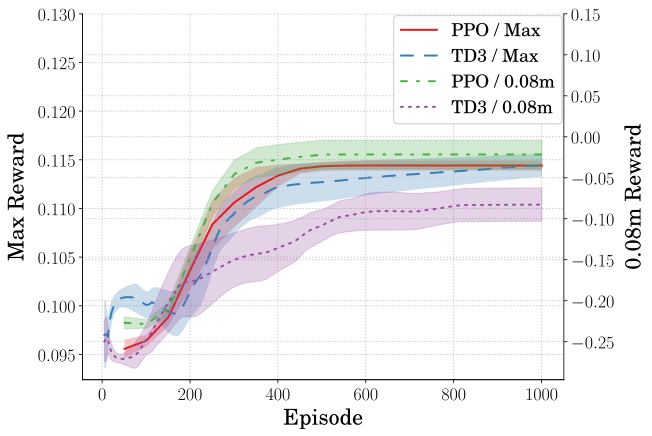
\includegraphics[width = 3in]{figures/ppo_vs_td3/avg_rew_comp.png}  
        \caption{Reward Received During Training}
        \label{fig:rew_vs_step}
        \end{center}
        % \vspace{-4mm}
        \end{figure}
%

The average and standard deviation of the spring constant and damping ratio design parameters the agents selected during training are shown in Figures~\ref{fig:spring_vs_step} and~\ref{fig:zeta_vs_step}. 
These figures show that the PPO and TD3 Algorithm on average converge to a similar result when training for Maximum height. However, the variation in the standard deviation of the parameter choices between the PPO agents, show that each agent's parameter choice varied greatly between episodes. This implies a higher preference for exploration in the PPO agents than the TD3. The larger standard deviation of the TD3 algorithms does not demonstrate the algorithm's preference for exploration, instead it shows that agents trained with TD3 algorithm converged on solutions with more significant differences.
When the agents were trained to jump to a specific height, the two algorithm's agents converged on different solutions. Additionally, the standard deviation of the spring constant learned by both algorithms agents, and the damping ratio learned by the PPO algorithm agents, are significantly larger than when the agents were trained for maximum height. This is due to there being a wider range of possible solutions to achieve the specified height of 0.08m.
%
\begin{figure}[tb]
        \begin{center}
        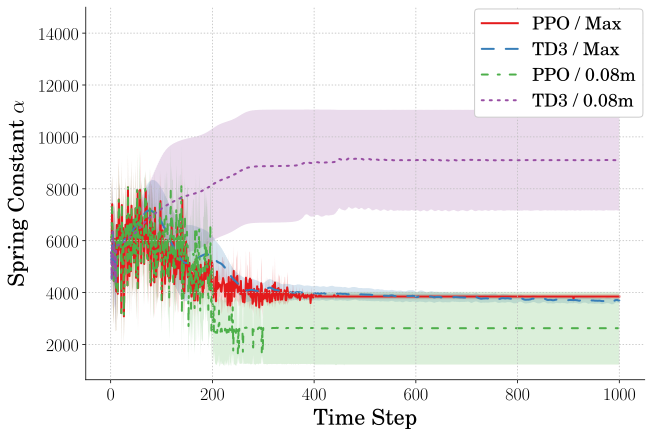
\includegraphics[width = 3in]{figures/ppo_vs_td3/avg_spring_comp.png}  
        \caption{Spring Constant Selected During Training}
        \label{fig:spring_vs_step}
        \end{center}
        % \vspace{-4mm}
        \end{figure}
%
\begin{figure}[tb]
        \begin{center}
        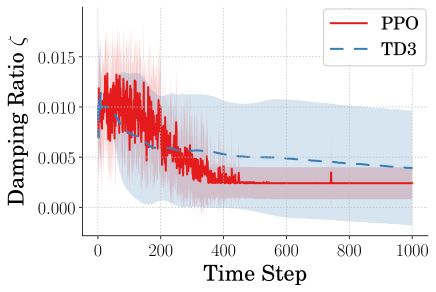
\includegraphics[width = 3in]{figures/ppo_vs_td3/avg_zeta_comp.png}  
        \caption{Damping Ratio Selected During Training}
        \label{fig:zeta_vs_step}
        \end{center}
        % \vspace{-4mm}
        \end{figure}

\subsection{Average Design Performance}
%
\begin{figure}[tb]
        \begin{center}
        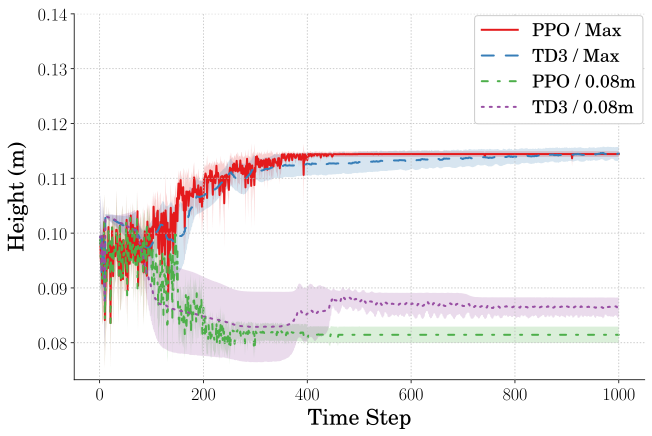
\includegraphics[width = 3in]{figures/ppo_vs_td3/avg_height_comp.png}  
        \caption{Response of Average Optimal Designs}
        \label{fig:height_vs_time}
        \end{center}
        % \vspace{-4mm}
        \end{figure}

Figure~\ref{fig:height_vs_time} shows the jumping performance of the mean designs learned for both algorithms tested. The peak heights achieved can be compared again to Figure~\ref{fig:spring_zeta_height} to show that the agents learned designs nearing those achieving maximum performance. The figure also shows that the agents trained using the PPO algorithm was able to better
match the specified jump height of 0.08m, where the TD3 agents overshot the specified height.

%%%%%%%%% CONCLUSION

\section{Conclusion}
\label{sec:conclusion}
The monopode model was used in conjunction with a predetermined control input to compare the performance of the TD3 and PPO reinforcement learning algorithms at finding optimal performing design parameters regarding jumping performance. This work was done in part to determine if reinforcement learning could be used as the mechanical design learner for an intelligent concurrent design algorithm. It was shown that when training for maximum jump height the algorithms train agents with similar maximum heights, however the standard deviation of the PPO agents designs is smaller. 
Additionally, when training for a specified height the PPO algorithm outperformed the TD3 algorithm, having a higher average reward.


%%%%%%%%% REFERENCES
{\small
\bibliographystyle{ieee_fullname}
\bibliography{C:/Users/andre/Documents/BibTeX/CRAWLAB}
}

%%%%%%%%% APPENDIX
\appendix
%%%%%%%%% Learning Rate

\section{Learning Rate}
\label{app:lr_changes}
\begin{figure}[b]
\begin{center}
        \includegraphics[width=3in]{figures/comp_learning_rate/avg_rew_ppo.png}
        \caption{Reward Due to Changes in PPO Learning Rate}
        \label{fig:ppo_rew}
\end{center}
% \vspace{-4mm}
\end{figure}

\begin{figure}[tb]
\begin{center}
        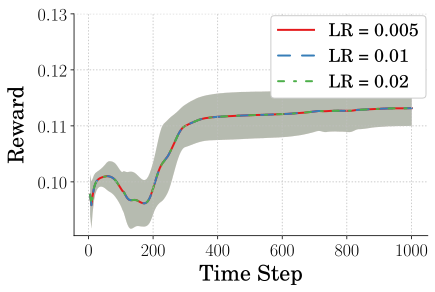
\includegraphics[width=3in]{figures/comp_learning_rate/avg_rew_td3.png}
        \caption{Reward Due to Changes in TD3 Learning Rate}
        \label{fig:td3_rew}
\end{center}
% \vspace{-4mm}
\end{figure}
        
In the process of this project the effects of learning rate on the PPO and TD3 Algorithms were explored.
Figures~\ref{fig:ppo_rew} and \ref{fig:td3_rew} show that the Time Steps needed for the PPO algorithm to converge is very sensitive to the choice in learning rate, it also shows that the overall mean and standard deviation of the rewards is sensitive. On the other hand, Td3 does not appear to be at all sensitive to changes in the learning rate, at least not in the range of learning rates explored in this study.

%%%%%%%%% Update Rate
\section{Update Rate}
\label{app:ur_changes}

\begin{figure}[b]
\begin{center}
        \includegraphics[width = 3in]{figures/ppo_n_steps/avg_rew_ppo.png}
        \caption{Reward Due to Changes in N Steps}
        \label{fig:n_steps}
\end{center}
% \vspace{-4mm}
\end{figure}

In addition to learning rate the effects of the update rate on PPO was explored. This study found an update rate of one update per 50 time steps to be optimum. The results shown in Figure~\ref{fig:n_steps} show that an update rate of 100 is to slow as the algorithm is unable to converge by the 1000th Time Step. The figure also shows that updating every 10 steps is also a poor choice. This is because the
algorithm is forced to make updates on small batch sizes.

\end{document}
